\section{Análise preliminar}

Utilizarei a biblioteca \emph{sympy} do \emph{Python} para fazer a análise simbólica e numérica do circuito antes de montá-lo fisicamente.

Após terminar as análises compararei os resultados obtidos nas análises numéricas e em laboratório para verificar sua coerência.

\subsection{O circuito}

\begin{figure}[h]
    \centering
    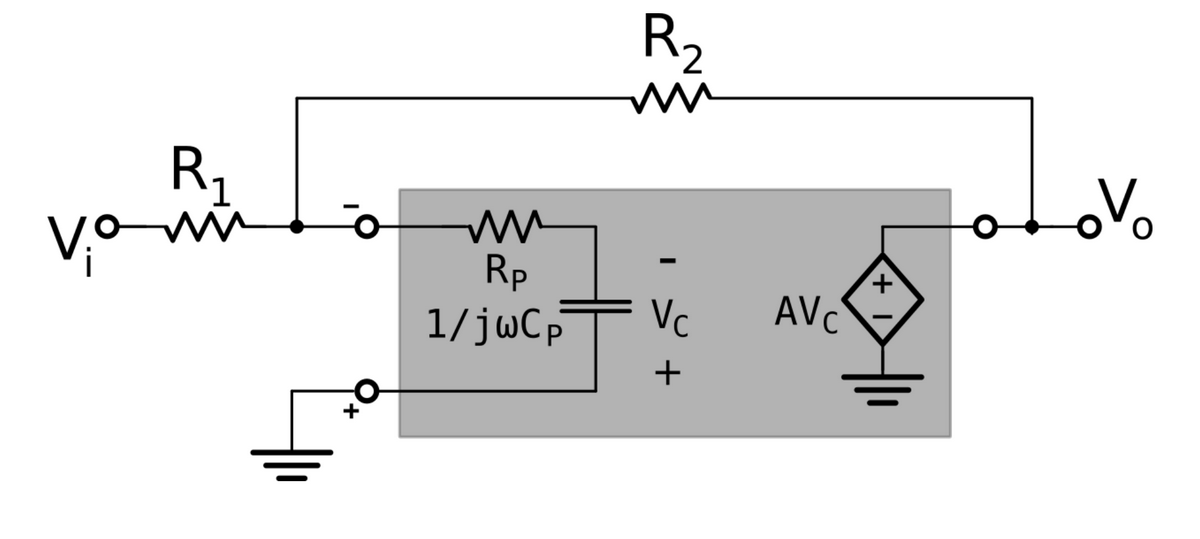
\includegraphics[width=1\columnwidth]{images/circuito.png}
    \caption{Circuito com amp op em configuração inversora.}
\end{figure}


\newpage
\subsection{Análise simbólica}


Podemos realizar a análise do circuito utilizando análise nodal.


\begin{equation}
    \begin{aligned}
        0       & = \frac{V_{a}}{R_{p} + \frac{1}{C_{p} j w}} + \frac{V_{a} - V_{o}}{R_{2}} + \frac{V_{a} - V_{i}}{R_{1}} \\
        - V_{c} & = \frac{V_{a}}{C_{p} j w \left(R_{p} + \frac{1}{C_{p} j w}\right)}                                      \\
        V_{o}   & = A V_{c}
    \end{aligned}
\end{equation}


Resolvendo as equações para $V_o$ obtemos que $V_o$ é dado por:


\begin{equation}
    - \frac{A R_{2} V_{i}}{A R_{1} + C_{p} R_{1} R_{2} j w + C_{p} R_{1} R_{p} j w + C_{p} R_{2} R_{p} j w
        + R_{1} + R_{2}}
\end{equation}


Aqui fazemos a seguinte simplificação $R_p >> R_1$ , $R_p >> R_2$, e $A >> 1$:


\begin{equation}
    V_o = - \frac{A R_{2} V_{i}}{A R_{1} + C_{p} R_{p} j w \left(R_{1} + R_{2}\right)}
\end{equation}


Com esta simplificação fazemos $\frac{V_o}{V_i}$ para obter a função transferência $H\left(jw\right)$:


\begin{equation}
    H\left(jw\right) = - \frac{A R_{2}}{A R_{1} + C_{p} R_{p} j w \left(R_{1} + R_{2}\right)}
\end{equation}


Agora podemos reorganiza-la no formato de um filtro passa-baixa para achar o ganho $K$, e a frequência de corte $w_c$:


\begin{equation}
    \begin{aligned}
        H(jw) & = - \frac{K w_c}{jw + w_c} \\
        w_p   & = \frac{1}{R_p C_p}        \\
        K     & = \frac{R_2}{R_1}          \\
        w_c   & = \frac{A w_p}{1 + K}
    \end{aligned}
\end{equation}


Podemos também achar o valor absoluto de $H(jw)$:


\begin{equation}
    \lvert H(jw) \rvert = \frac{\left|{K w_{c}}\right|}{\sqrt{w^{2} + w_{c}^{2}}}
\end{equation}


\subsection{Análise numérica}


Aqui utilizaremos as equações (5) e (6) para implementar o circuito discutido acima com dois conjuntos de valores, os conjuntos diferem apenas em seu $R_2$


Para ambos circuitos utilizaremos os seguintes valores:


\begin{equation}
    \begin{aligned}
        R_1 & = 4.7k \varOmega \\
        w_p & = 2 \pi 1k rad/s \\
        A   & = 10^5
    \end{aligned}
\end{equation}


\subsubsection{Circuito 1}


Neste utilizaremos o valor  $R_2 = 22k$:


Isto nos dá:


\begin{equation}
    \begin{aligned}
        K   & = 4.68                     \\
        w_c & = 1.10 \times 10^{6} rad/s
    \end{aligned}
\end{equation}


\begin{center}
    \begin{tabular}{ |c|c|c| }
        \hline
        freq rad/s & freq Hz         & $\lvert H(jw) \rvert$ \\
        $0.5 w_c$  & $88014.98 Hz$   & 4.19                  \\
        $w_c$      & $176029.96 Hz$  & 3.31                  \\
        $2 w_c$    & $352059.93 Hz$  & 2.09                  \\
        $4 w_c$    & $704119.85 Hz$  & 1.14                  \\
        $10 w_c$   & $1760299.63 Hz$ & 0.47                  \\
        $20 w_c$   & $3520599.25 Hz$ & 0.23                  \\
        $40 w_c$   & $7041198.50 Hz$ & 0.12                  \\
        \hline
    \end{tabular}
\end{center}


\subsubsection{Circuito 2}


Neste utilizaremos o valor  $R_2 = 560k$:


Isto nos dá:


\begin{equation}
    \begin{aligned}
        K   & = 119.15      \\
        w_c & = 52295 rad/s
    \end{aligned}
\end{equation}


\begin{center}
    \begin{tabular}{ |c|c|c| }
        \hline
        freq rad/s & freq Hz      & $\lvert H(jw) \rvert$ \\
        $0.5 w_c$  & $4161.50 Hz$ & 106.57                \\
        $w_c$      & $8323 Hz$    & 84.25                 \\
        $5 w_c$    & $41615 Hz$   & 23.37                 \\
        $20 w_c$   & $166460 Hz$  & 5.95                  \\
        $50 w_c$   & $416150 Hz$  & 2.38                  \\
        $200 w_c$  & $1664600 Hz$ & 0.60                  \\
        $500 w_c$  & $4161501 Hz$ & 0.24                  \\
        $1000 w_c$ & $8323003 Hz$ & 0.12                  \\
        \hline
    \end{tabular}
\end{center}


\newpage


\subsubsection{Gráfico dos exemplos}


\begin{figure}[h]
    \centering
    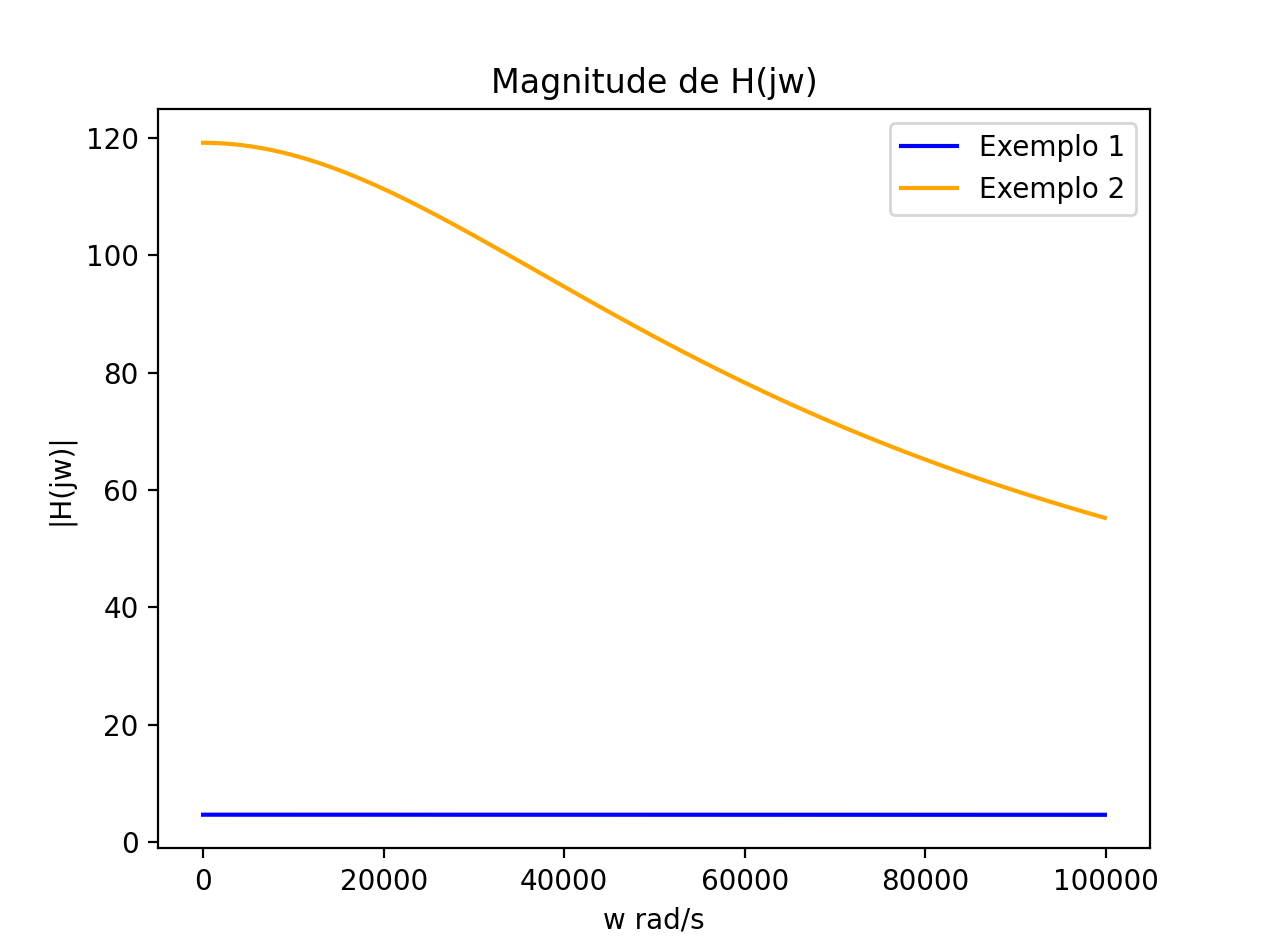
\includegraphics[width=1\columnwidth]{images/plot_bode.png}
    \caption{Gráfico da magnitude pela frequência dos exemplos 1 e 2.}
\end{figure}


\newpage

